\subsection{Theoretische Grundlagen}
Die Schärfentiefe (engl. depth of field (DOF)) beschreibt die Distanz,
beziehungsweise einen Entfernungsbereich,
in welcher ein Objekt scharf abgebildet wird.

\begin{figure}[h!]
  \centering
  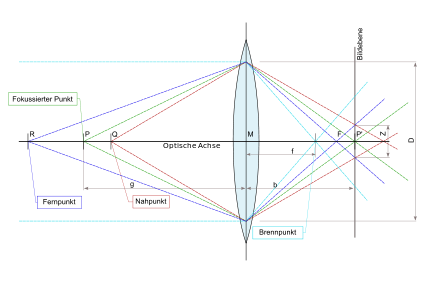
\includegraphics[width=.6\textwidth]{Posten_1_theo}
  \caption{Strahlengänge zur Bestimmung der Schärfentiefe mit Fernpunkt im Endlichen \cite{ref:wiki:schaerfentiefe}}
  \label{fig:p1theo}
\end{figure}

Zur Berechnung der Schärfentiefe werden die Brennweite $f$, die Blendenzahl $k$,
die Gegenstandsweite $g_s$ und die grösse des Zerstreuungskreis $Z$ benötigt.
Wie in Abbildung \ref{fig:p1theo} ersichtlich, gibt der Zerstreuungskreis $Z$ an,
wie gross eine Punktquelle auf der Bildebene abgebildet wird.
Da die Bildebene mit der Auflösung des Bildsensors abgetastet wird,
sind Kreise kleiner als die Pixelgrösse kaum wahrnehmbar,
das heisst die Aufnahme wird noch immer scharf.

Für die Bestimmung der Schärfentiefe, respektive des Nah- und Fernpunktes,
wird die hyperfokale Entfernung benötigt.
Diese beschreibt, auf welche endliche Entfernung fokusiert werden muss,
so dass der Fernpunkt im Unendlichen liegt.

\begin{equation}
  g_h=\frac{f^2}{kZ}+f
\end{equation}

Der Nahpunkt lässt sich wie folgt berechnen: 
\begin{equation}
  g_n=\frac{g_s}{1+\frac{g_s-f}{g_h-f}}
\end{equation}

Die Berechnung der Fernpunkts benötigt nur eine Anpassung eines Vorzeichens:
\begin{equation}
  g_f=\frac{g_s}{1-\frac{g_s-f}{g_h-f}}
\end{equation}

\newpage
\subsection{Versuchsaufbau}
Benötigtes Material:
\begin{itemize}
\item Kamera Basler A1300-30gc
\item Objektiv Computar 25mm f1.4:16
\item Objektiv Computar 16mm f2:16
\end{itemize}

Der Studentenausweis wird wie in Abbildung \ref{fig:p1auf} vor der Kamera aufgestellt.
Mit beiden Objektiven wird die Schärfentiefe mit unterschiedlichen Blendenstufen untersucht.

\begin{figure}[h!]
  \centering
  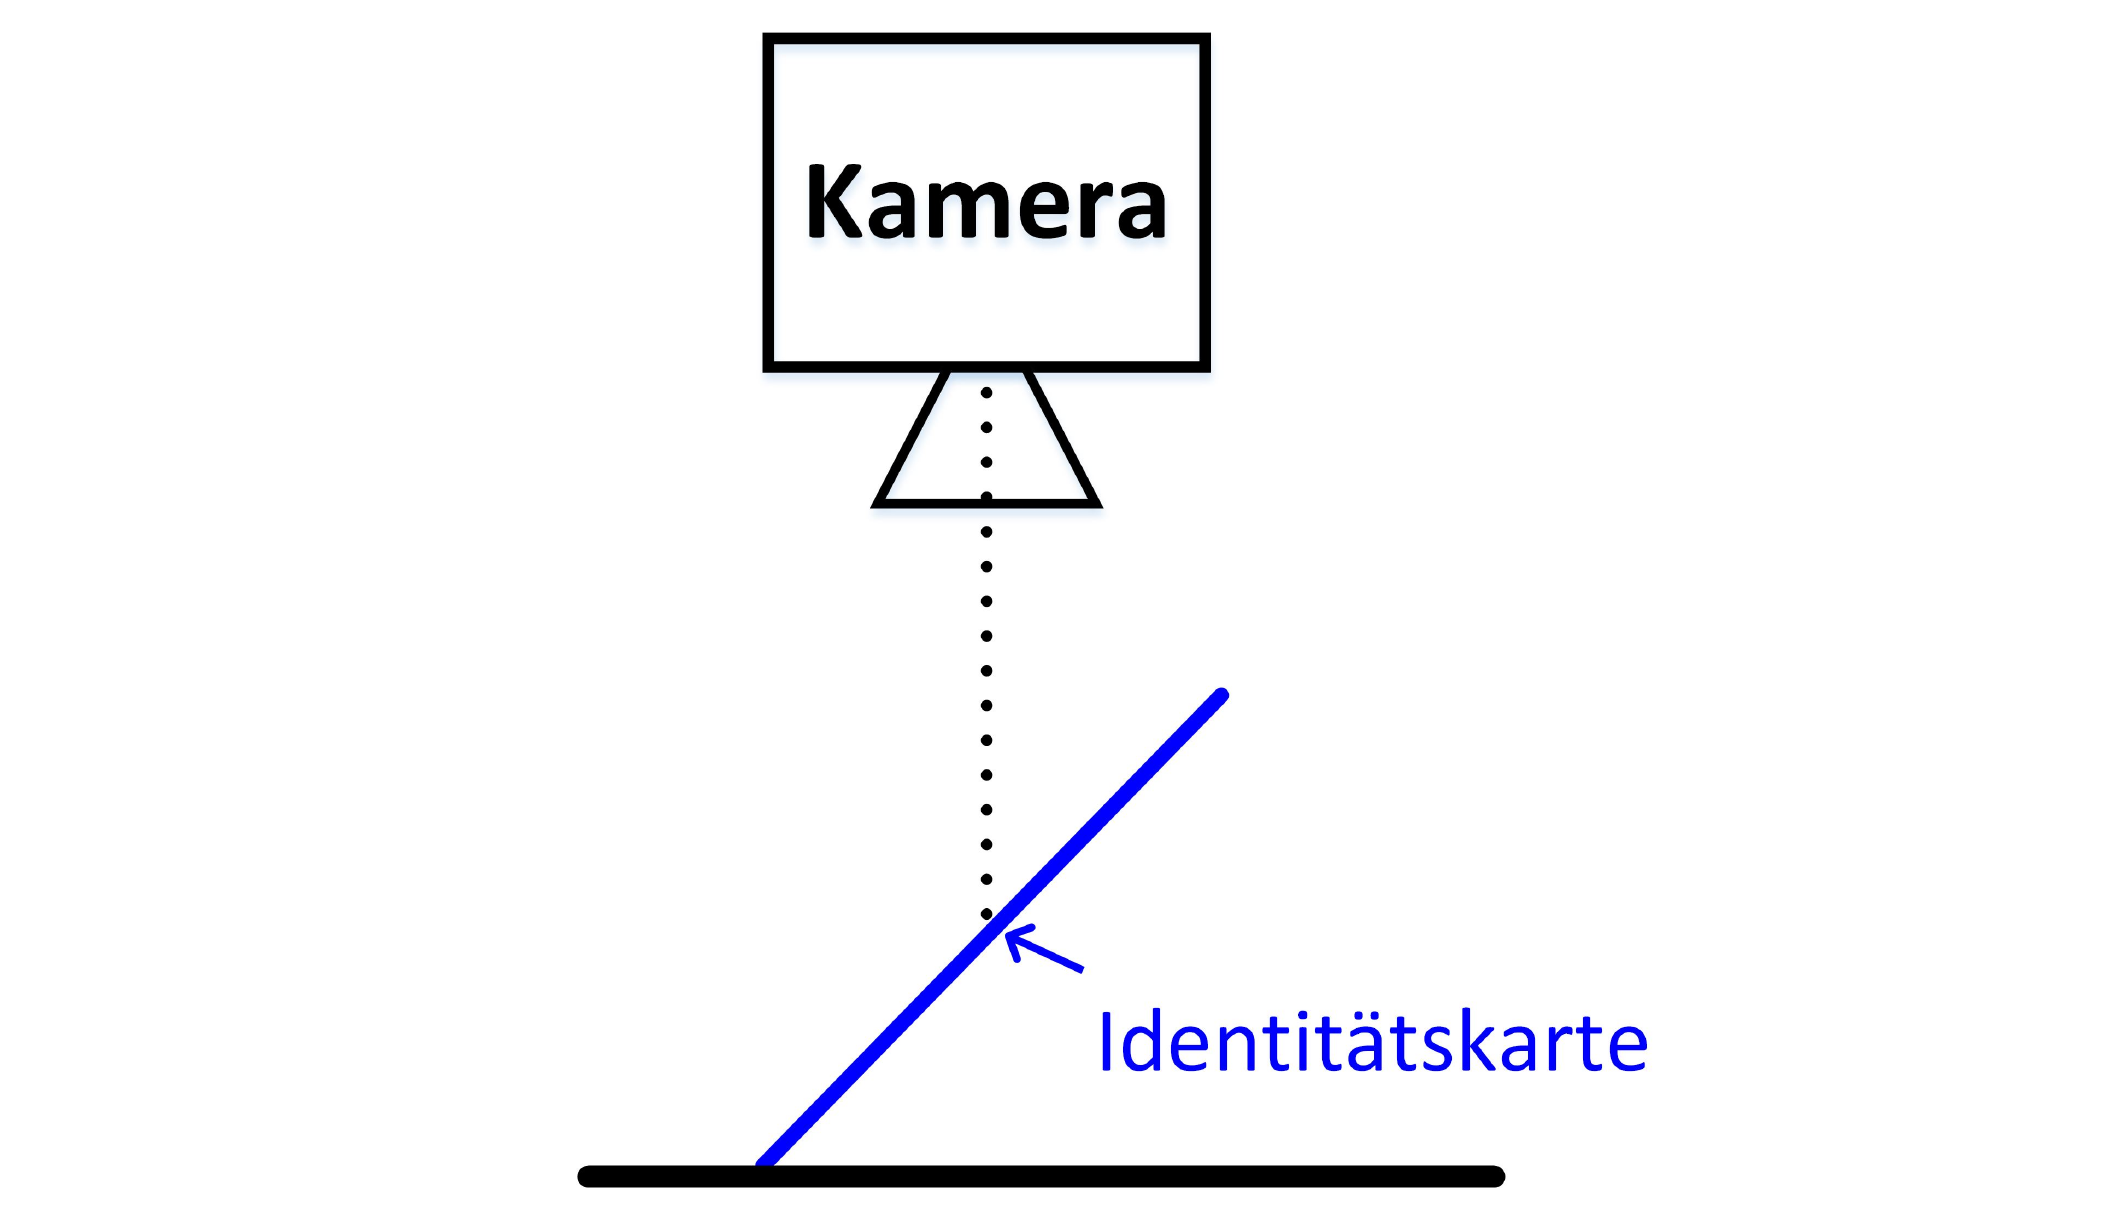
\includegraphics[width=.6\textwidth]{Posten_1_aufbau}
  \caption{Versuchsaufbau \cite{ref:bver:stefan}}
  \label{fig:p1auf}
\end{figure}

\subsection{Ergebnisse}
\subsubsection{Testbild mit Brennweite 25mm und f1.4}
\begin{wrapfigure}[5]{L}{.6\textwidth}
  \centering
  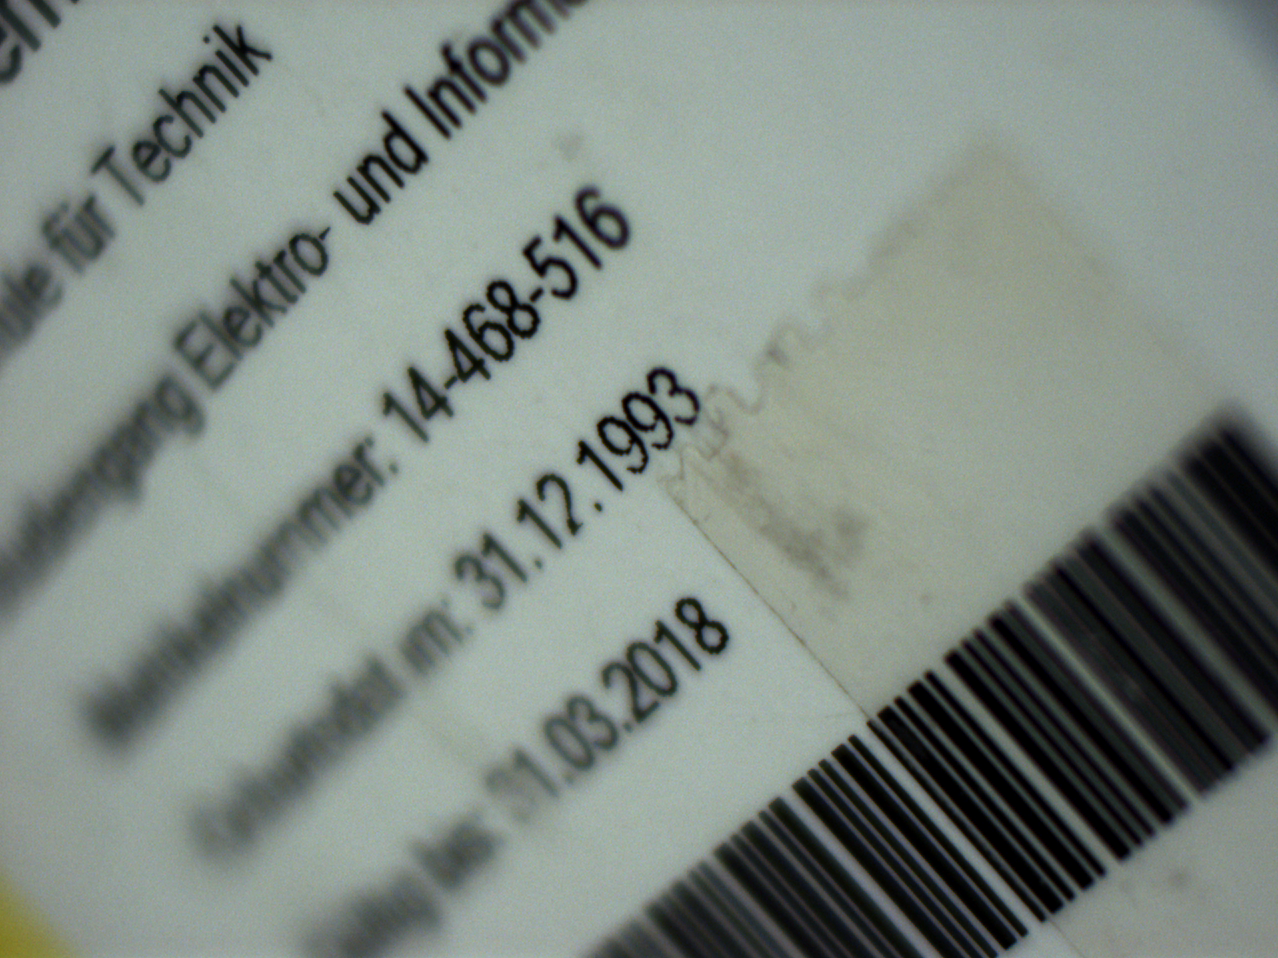
\includegraphics[width=.6\textwidth]{Posten_1_img_1}
  \caption{Studentenausweis mit Brennweite 25mm f1.4}
  \label{fig:b25f1.4}
\end{wrapfigure}

~\\[2em]
Einstellungen:\\
\begin{tabular}{l l}
  Brennweite $f$:        &  $25$mm\\
  Blendenzahl $k$:       & 1.4 \\
  Distanzscharf $g_s$    & 140mm \\
  Zerstreuungskreis $Z$: & $0.00375$mm\\
\end{tabular}

~\\[10em]

\[
  g_h=\frac{25^2}{0.00375*1.4}+25=119072.61904\;\text{mm}
\]
\[
  g_n=\frac{140}{1+\frac{140-25}{g_h-25}}=139.86\;\text{mm}
\]
\[
  g_f=\frac{140}{1-\frac{140-25}{g_h-25}}=140.14\;\text{mm}
\]

\subsubsection{Testbild mit Brennweite 16mm und f2}
  \begin{wrapfigure}[5]{L}{.6\textwidth}
    \centering
    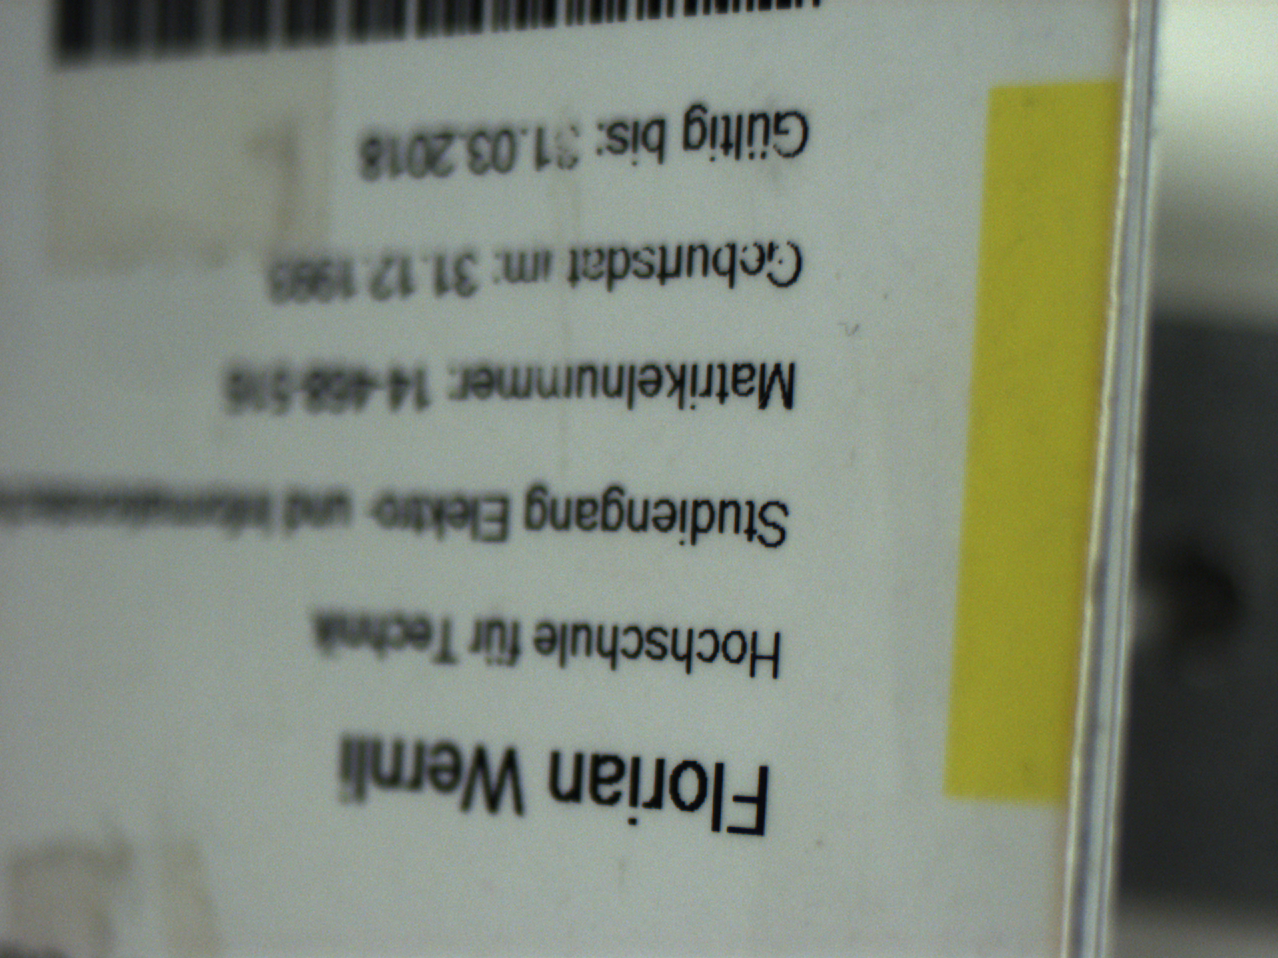
\includegraphics[width=.59\textwidth]{Posten_1_16mm_1}
    \caption{Studentenausweis mit Brennweite 16mm f2}
    \label{fig:b25f2}
  \end{wrapfigure}

  ~\\[2em]
  Einstellungen:\\
  \begin{tabular}{l l}
    Brennweite $f$:        & $16$mm\\
    Blendenzahl $k$:       & 2 \\
    Distanzscharf $g_s$    & 140mm \\
    Zerstreuungskreis $Z$: & $0.00375$mm\\
  \end{tabular}

  ~\\[10em]

\[
  g_h=\frac{16^2}{0.00375*2}+16=34149.3333\;\text{mm}
\]
\[
  g_n=\frac{140}{1+\frac{140-16}{g_h-16}}=139.49\;\text{mm}
\]
\[
  g_f=\frac{140}{1-\frac{140-16}{g_h-16}}=140.51\;\text{mm}
\]

\subsection{Erkenntnisse}

Die Schärfentiefe ist bei weit entfernten Objekten grösser, da die eingestellte Schärfe sich der hyperfokalen Entfernung nähert, beziehungsweise der Einfallswinkel der Strahlen weniger stark mit der Distanz variiert.

Der Versuch zeigt sehr gut, dass eine Verbesserung der Schärfentiefe durch die Verkleinerung der Blendenöffnung erfolgen kann.
Die künstliche Vignettierung verkleinert den Unschärfekreis.
Da aber weniger licht auf den Sensor fällt, muss das Signal mehr verstärkt werden,
wodurch das Rauschen erhöht wird.

Nicht direkt aus dem Versuch aber aus der Formel ist ersichtlich, dass eine kleiner die Brennweite der Optik und damit ein kleiner der Sensor positiv zur Schärfentiefe beitragen, ebenso wie eine grössere Pixelgrösse.